\chapter{Implementation of Techniques to Mitigate Catastrophic Forgetting into Cognitive Space Communications Engine}\label{ch:methods}
\par In the following chapter, both software and hardware details of the test platforms used will be described. First, details about the software platforms will be included. This initially describes aspects of the software that are independent of the programming languages. Then, the language-dependent details will be provided. The CE was first implemented in MATLAB, to verify functionality. This was then ported to C++ using the MLPack library. Details about implementation in both languages will be described, both for the baseline implementation (CE-LM) and the two modified training methods (CE-RLM and CE-NSE). Once the software is described, the hardware setups for ground testing and flight testing will be described. Finally, the postprocessing will be briefly discussed.

\section{Software Methods}
\par The architecture of the CE is independent of the implementation language, and will be described first. Following that, the specific elements of MATLAB implementation and C++ implementation will be explained.
\subsection{CE Details}
\par The architecture of the CE follows the SARSA algorithm described in Algorithm \ref{code:bg_SARSA}. A flow diagram illustrating how data passes through the CE is shown in Figure \ref{fig:ceDataFlow}. There are a couple differences between the CE and classic SARSA: the replacement of the Q-table with an MLP and the use of a separate MLP to guide the exploration of the network. The replacement of the Q-table with an MLP transforms the Q learning into a Deep-Q Network.

\begin{landscape}
\begin{figure}[ht]
\includegraphics[width=\paperwidth]{figures/rough_flow_diagram.eps}
\caption{placeholder figure for CE block diagram}\label{fig:ceDataFlow}
\end{figure}
\end{landscape}
\par The CE begins by randomly selecting actions and observing the results of these actions, storing unique action-reward pairs in a history buffer. In this experiment, the action is the specific configuration of PHY parameters, and the reward is a fitness score created by taking a weighted combination of different evaluation metrics. These metrics include thoughput, spectral efficiency, bandwidth used, power consumed on transmit, bit error rate (BER), and DC power consumed. Throughput, spectral efficiency, and bandwidth are all calculated based on the chosen set of PHY parameters, while DC power consumed and transmit power consumed are measured. A model of BER based on the other metrics is used as an estimate for BER that doesn't require more than one sample to confirm. Each parameter gets scaled from 0 to 1 based on the values that can be expected from each input. Then, they get combined in a weighted manner to produce the resulting fitness score. The importance of each metric is hard to determine, and can change depending on what priorities the system currently has. Six different weight combinations were arbitrarily selected to represent plausible use cases, and are shown in Table \ref{table:fitMissions}. Once the fitness score is calculated, the action-reward pair is stored in the history buffer until it fills up, after which the Explore and Exploit MLPs get trained. During initial training, the CE uses an action that is fairly robust, to ensure a baseline result. Once done training, the CE has completed its startup process.
\begin{table}[ht]
\centering
\begin{tabu} to 1.1\textwidth{|X[c]|X[c] X[c] X[c] X[c] X[c] X[c]|}
	\hline 
	Mission Name & Throughput&BER&Target BW&Spectral Efficiency&TX Efficiency&DC Power Consumed\\
	\hline
	Emergency& 0.1 &0.8&0.025&0.025&0.025&0.025 \\
	Cooperation&0.05&0.05&0.4&0.4&0.05&0.05\\
	Power Saving&0.05&0.05&0.05&0.05&0.3&0.5\\
	Balanced&1/6&1/6&1/6&1/6&1/6&1/6\\
	Launch&0.2&0.4&0.1&0.1&0.1&0.1\\
	Multimedia&0.5&0.3&0.05&0.05&0.05&0.05\\
	\hline
\end{tabu}
\caption{Table containing different ways fitness score can be weighted.}
\label{table:fitMissions}
\end{table}
\par For the first step after training, the exploration threshold $\epsilon$ is set to 1, forcing an explore During each following step, the $\epsilon$ value is recalculated by taking the inverse of an incrementing counter. When this value passes a threshold, the counter is reset and exploration is again forced. After $\epsilon$ is updated, a number is drawn from uniformly random distribution $\mathcal{U}(0,1)$. Then, if this number is less than $\epsilon$, an explore iteration is triggered. Otherwise, an exploit iteration is triggered.
\par In the case of an exploration, all actions in the action space, as well as the normalized observed SNR, are used as inputs to the Explore MLP block. The MLP returns a predicted fitness score for each action. From this, the actions are split up into two groups: actions that have a fitness score greater than the threshold and actions that have a fitness score less than the threshold. Then, with a 95\% probability, an action is randomly selected from the group of actions with a greater fitness score than the threshold. The 5\% probability of selecting from the other group of actions allows for exploration of areas that the Explore MLP block may have misinterpreted or areas that have been insufficiently explored.
\par In the case of exploitation, The normalized observed reward values of the last action are used as inputs to the exploit MLP block. Each member of the Exploit block has 6 component MLPs. Each component MLP corresponds to a normalized tuneable parameter. These six output values are then denormalized to get the actual output actions.
\par Regardless of if the action was chosen through exploration or exploitation, it is transmitted to the SDR platform (either in simulation or reality). The $E_s/N_0$ of the message is then received.  Power consumed, power efficiency, bandwidth used, throughput, BER, and spectral efficiency are then calculated, based on the action chosen and the $E_s/N_0$. Once these are all present, a fitness score is calculated depending on the mission that the CE is configured to run. 
\par If the fitness value is greater than the maximum previously observed value, it becomes the new maximum observed value. If this value was achieved during exploration, the performance values are the next input to the exploit network. If the value is less than the maximum value and was chosen by exploitation, a new set of logic is followed. A value $e_p$ is kept, representing the maximum fitness value while accounting for slow drift in fitness value responses resulting from slow-changing environmental properties. If the action taken was the same as the previous action, and the observed fitness is less than $0.9 e_p$, then it is assumed the environment has undergone a rapid shift. The history buffer is reset and the system is reset to the initial state, where it randomly explores until the history buffer is filled.  If the observed fitness is less than $0.9 e_p$ but a different action was chosen, then the CE finds the best performing action from the history buffer and uses that action. Otherwise, if the observed fitness is greater than $0.9 e_p$ and is not the first sample in the buffer, the new action is accepted. If the observed fitness is greater than $0.9 e_p$ and no quick recover has occurred, the last known action is chosen as the new action to take. Finally, if the observed fitness is greater than $e_p$, $e_p$ gets updated, and the last exploitation action gets chosen. This logic path is illustrated in figure \ref{fig:action_acceptance_protocol} 


\begin{figure}[ht]
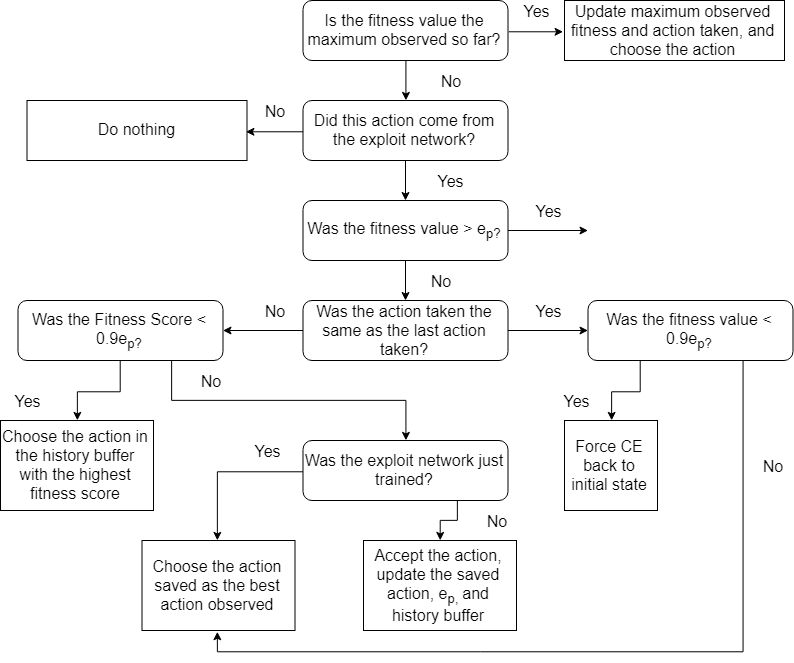
\includegraphics[width=\textwidth]{figures/action_acceptance_protocol.png}
\caption{Flow diagram illustrating the logic process of filtering the action choice based on previously seen results. This logic allows the CE to catch if major changes prompt a retraining period.}
\end{figure}

\par Once the action-choosing logic has occurred, the observed fitness values are added to the history buffer. If the action chosen is unique to any action in the buffer, the results are directly added to the history buffer. Otherwise, the CE updates the observed fitness value of the action in the buffer. If the history buffer is full, the explore and exploit networks get trained. In C++, the training process occurs in parallel with the rest of the CE so that the Explore and Exploit networks can continue to get used during training. The MATLAB simulation does not have the parallel training, but timing information from the simulation is not used. If the history buffer isn't full, the next iteration of the CE occurs.
\par Training occurs in two phases, one for explore and one for exploit. During each phase, data from the history buffer is randomly split up into training and testing sets. Then, the training algorithm is applied, whether it is LM, RLM, or NSE. Details of the implementation of each will be described in the language-specfic sections. 
\par The Explore and Exploit MLPs had different architectures, but maintained some similarities. Both used logarithmic activation functions, as well as a linear output function. The Explore MLP was composed of 3 layers. The input layer takes 7 inputs, The first hidden layer has 7 nodes, the second hidden layer had 50 nodes, and the output layer has 1 node. The Exploit MLP was actually 6 different MLPs, one for each parameter to be predicted. Each sub-MLP has 2 layers, with 7  inputs, 20 nodes on the first hidden layer and 1 output. 
\par In the past, each weight was initialized using MATLAB's default initialization method, Nguen-Widrow initialization \cite{placeholderCitation}. However, due to convergence issues the RLM method encountered while using this, the weight initialization was changed to the Glorot (Xavier) initialization technique\cite{glorot_training}, which sets weights by drawing from gaussian distribution $\mathcal{N}(0,\sigma^2)$, where:
\begin{align*}
	\sigma^2 &= \frac{2}{n_{in}+n_{out}}
\end{align*} 
\par $n_{in}$ and $n_{out}$ are the number of input and output nodes in the network.
\subsection{Simulation}
\par Prior to this thesis, the CE was prototyped in MATLAB by Paulo Ferriera\cite{paulo_theory_paper}. It was developed in MATLAB 2015a, using the Parallel Computing Toolbox and the Neural Network Toolbox. It is important to note that the Statistics and Machine Learning toolbox was used and not the Deep Learning toolbox. Both toolboxes are able to create the CE, but have different interfaces. The following section will describe in summary the structure of the baseline simulation, as well as the modifications required to implement RLM and NSE. The full MATLAB code base can be found in Appendix (\ref{app:MatlabCode}).
\par For all learning methods, the MATLAB neural network structure was used as the foundation. However, for RLM and NSE, the framework was augmented with training functions specific to each algorithm. Most of the previous implementation of the CE was untouched during the thesis. Indeed, the only part that had major changes is the training function, which is abstracted away by default. 
\par By the nature of RLM, there are a handful of parameters and intermediate values that need to be kept track of. This was done using a matlab struct, RecurseMatrix, found in Appendix \ref{app:MatlabCode:recurseMatrix}. It contains the current Gradient, time, $P$ matrix, $\rho$, $S$, $\alpha$, and the size of a batch to be trained. Beyond that, the algorithm described in \ref{bg:RLM_ref} is followed in a straightforward way.   
\par  The implementation of Learn++.NSE was modified from the version provided by \cite{placeholderCitation}. When working with the US government, International Traffic in Arms Regulations (ITAR) constraints must always be considered. The code provided by \cite{placeholderCitation} uses a GNU General Public License (GPL), which requires that the source of a program using the library is accessible under the same license. This poses issues to ITAR-controlled code. However, the MATLAB simulation has no ITAR sensitive material, so the license did not matter in this case.
%https://github.com/gditzler/IncrementalLearning/tree/master/src \textbf{\textit{DON'T FORGET TO FIX THIS INTO AN ACTUAL CITATION LOL}}. 
\par The main changes to the code provided by \cite{placeholderCitation} involved adjusting the structure to fit a regression problem instead of a classification problem. Adaboost.R1 was used as a reference point in doing this adjustment, as it is similar in operation, if not how it weighs samples \cite{adaboostPaper}. The cross-entropy loss function that the standard Learn++.NSE algorithm used \cite{learnNseIntro} was replaced by mean squared error (MSE). In addition, during prediction the result was a weighted average of the ensembles, instead of a weighted majority vote. Other than the changes necessary for adapting Learn++.NSE to regression, not much was changed, beyond a handful of extra hyperparameters. 

\subsection{C++}
\par The software architecture used in ground and flight testing was initially introduced by the authors in \cite{tim_implementation_paper}. In order to ensure generality, performance, and reusability, an Object-Oriented programming language was most suitable. C++ was chosen, both for performance and for some of the constructs in the C++11 standard. In addition, many helpful open-source C++ libraries exist. The software was designed and compiled in an Ubuntu 16.04 Linux VM, but was designed to be recompilable for any x86-based operating system, and can, with work, be used with most processor types that have a C++ compiler.
\par In the design of the CE, drivers for the multiple modems needed to be created. These drivers are restricted by ITAR, ruling out the use of many libraries with "copyleft" licenses, such as the GNU GPL. This greatly reduces the pool of possible libraries to use. 
\par Despite the wide variety of publicly available ML libraries, many of them do not have APIs for lower-level languages such as C/C++. While this is rapidly changing with the development of embedded ML applications, at the time of the initial CE constructiothe selection of C++-compatible libraries was small \cite{tim_implementation_paper}. Furthermore, many of the existing C/C++ libraries lacked in-depth documentation for the lower-level APIs, had very complex build processes, or were built for larger, more complex applications (such as deep, convolutional NNs). 
\par MLPack \cite{placeholderCitation} was the library chosen to implement the MLPs in the CE. Because of the time of development the version used was 2.1.1. Since then, MLPack has revamped its ANN architecture, so the library version is important when attempting to replicate these results. MLPack is built on top of Armadillo 7.600.2 \cite{placeholderCitation}, so Armadillo was used for self-written matrix/vector operations and storage as well. By doing this, the interfacing between self-written components and MLPack was simple. 
\par In order to simplify the interfacing that the CE has to do with Ethernet and UDP/IP for communication with modems (described in Section \ref{mthds:hardware}), the Boost.ASIO \cite{placeholderCitation} library was used. This library abstracts away any operating system-specific constructs for handling sockets.
\par Finally, the Boost.Serialization \cite{placeholderCitation} library was chosen for saving/resuming CE states. 
\begin{figure}
\caption{\textbf{\textit{[baseline implementation, get figure 2 from Tim's paper]}}}
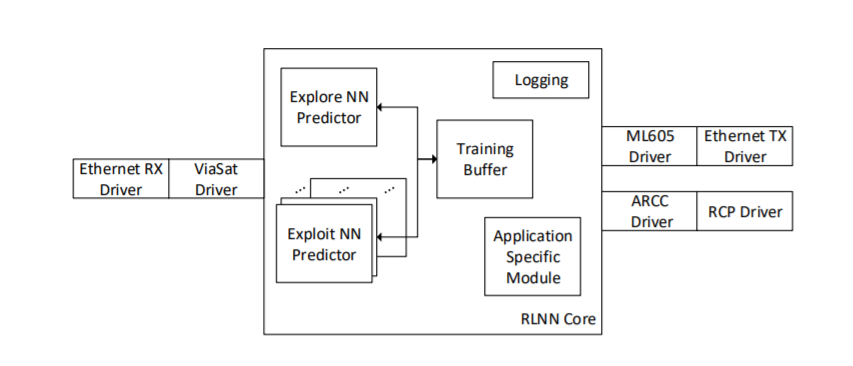
\includegraphics[width=\textwidth]{figures/driverList_tmp.png}
\label{fig:timOutlineBlocks}
\end{figure}
\par A block diagram of the CE is shown in Figure \ref{fig:timOutlineBlocks}. During the ground tests, the external drivers used are the ViaSat driver and the Advanced Radio for Cognitive Communications (ARCC) driver. The ViaSat modem is used to get the observed $Es/No$ value and the ARCC to simulate the response of the SCaN testbed from the action chosen by the CE. Since the ViaSat modem is connected through ethernet, an ethernet driver is necessary as well. During flight tests, the ARCC driver is replaced by the ML-605 BPSK driver, which also interfaces with the ethernet driver. The CE being tested resides in the RLNN Core section. The description of the RLNN Core will be split into three parts: the baseline method used in 2017, the changes required for the implementation of RLM, and the changes required for the implementation of Learn++.NSE.
\par The Explore and Exploit MLP ensembles were grouped into an NN Predictor object, allowing for references to the MLPack library to be abstracted out. In this implementation, any ensembles used were different solely on initialization of the weights. As such, both the Explore ensemble and Exploit ensembles had an effective ensemble size of 1. Within the NN Predictor object is the FeedForwardNetwork object, which implements the individual FFNN (MLP) and the implementation of Levenberg-Marquardt written by Timoty Hackett in \cite{tim_implementation_paper}. As described in \ref{bg:onlineLearning}, the CE uses online training. This required two NN Predictor models for each member of the ensemble, one to get trained and one for execution of the model. This allows for concurrent training and usage, only halting when weights are being copied over. Training occurs using one NN Predictor model, and then the weights get copied to the other NN Predictor model. 
\par The buffer of training data, which is common between Explore and Exploit NN Predictors, is implemented in a separate object. It holds the latest 200 unique actions. When training occurs, the buffer is split into training and validation sets, and is transformed for each type of MLP (as Explore and Exploit MLPs have different inputs and outputs). The Armadillo library is used to perform this splitting and transformation.
\par For the most part, the RLNN core of the CE is kept generic so that it can be applied to problems outside of communications. The Application Specific Module provides the satellite communications context for the RLNN core. It transforms communication metrics into the fitness scores that the rest of the RLNN Core uses. Any patches that change system behavior occur in this module as well. One example of this is the patch that limits transmit power changes to 1.5 dB steps. Another example is that the fitness scores are zeroed out when BER was measured to be 0.5, as this implies that the system had no communication between transmitter and receiver. 
\par The key differences between CE-RLM and CE-LM are located in the FeedForwardNetwork object. Here, the LM function was replaced by a function that runs RLM instead. Because of the additional parameters that RLM uses, a separate class called RecursiveLMHelper was used to contain the parameters and abstract the matrix math in the RLM updating process. In addition to these changes, CE-RLM used an ensemble of size 2 for the Exploit MLP structure. This was done to mitigate some of the instability of RLM. The Explore ensemble was kept at size 1, as each additional ensemble greatly increases execution time of the Explore MLP.
\par Unlike RLM, Learn++.NSE was mostly implemented as a modified version of NeuralNetwork Predictor, renamed LearnNSEPredictor. This is because the foundational MLP aspects of training are the same as the CE-LM. Where the difference occurs is the weighting of the samples that are being trained on and how the predictor is used. As such, the main changes occur in the train and predict functions. The algorithm is described in \ref{bg:nseSection}, and so will not be reiterated here. CE-NSE used a somewhat arbitrarily chosen Exploit ensemble of size 8. For similar reasons to CE-RLM, CE-NSE kept the Explot ensemble to size 1.
\par Post-processing the data gathered from the execution of the C++ implementations of the CE proved to be slightly more complicated than the MATLAB simulation, which had all relevant data easily exposed after running. The C++ CE was configured to keep a human-readable text log detailing the configuration of the CE. It also logged details about each iteration through the CE, including the start time, whether exploit or explore was chosen, the time that the action was chosen, the action chosen, the time an response was measured, the evaluation metrics received, the fitness score observed, and whether the network was training. The authors of \cite{tim_implementation_paper} provided a MATLAB script to parse the log files, which is included in Appendix \ref{app:MatlabCode:parser}. This parser generated figures that illustrate the results of a pass a time series as well as the amount of time it took to run the CE. It also generated MATLAB workspaces that contained useful information from the logs, which were used in the rest of the post-processing that occurred.


\section{Hardware Methods}\label{methods:hardware}
\par In the following section, the hardware used in the ground testing and the on-orbit testing.
\subsection{Ground Test Setup}

\par During the ground tests that were conducted during July of 2018, the test setup was very similar to that used in 2017 \cite{tim_implementation}.  Similarly to that work, a testbed at NASA GRC was used to create an emulation of the expected on-orbit environment. A simplified block diagram of the setup is shown in Fig. \ref{methods:groundTestFig}. The CE is contained in an Ubuntu 16.04 virtual machine on a Windows 7-based Dell T3600 Precision workstation. The VM was allocated 4 GB of dedicated memory, and shared all eight of the CPU cores (with hyper threading) with the host operating system. The CE is put on a private local area network with the ARCC test platform and the ViaSat DVB-S2 receiver. The CE transmits an action to the ARCC, which then transmitted DVB-S2 frames through a channel emulated by a variable attenuator, according to a measured SNR profile from a previous on-orbit experiment. The noise floor can be adjusted by the noise generator. All RF signals in this test were passed using coaxial cables, insetad of any antennas.
\begin{figure}[ht]
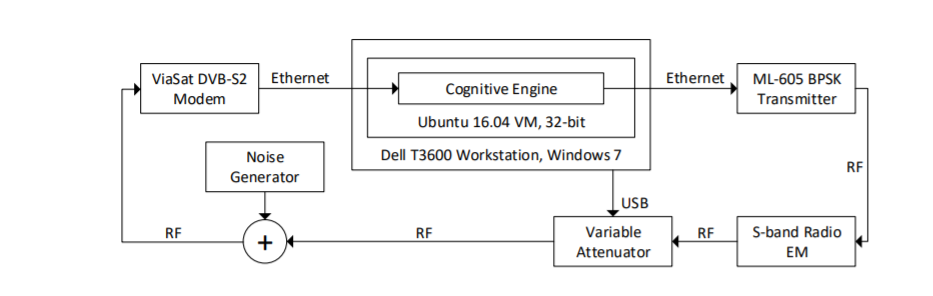
\includegraphics[width=\textwidth]{figures/groundHW_tmp.png}
\caption{\textbf{\textit{[Replace with actual figure once gotten from tim]}}}\label{methods:groundTestFig}
\end{figure} 

\subsection{Flight Setup}
\par The setup for on-orbit testing was identical to the setup used in 2017 \cite{tim_implementation}, which in turn used a setup initially used by previous NASA GRC collaborators. A simplified block diagram of the setup is shown in Fig. \ref{methods:flightTestFig}. In the chain, there are two DVB-S2 RX modems. The ViaSat modem was used for sending $E_s/N_0$ measurements at a rate of 100 Hz over UDP. The Newtec modem demodulates and decodes the actual frames coming in, and saves it to a binary file for postprocessing. During each dataframe, the CE saves the previous action tuple along with its performance. It then chooses the next action tuple, and sends the next action to the ML-605 BPSK modem, which then is used to uplink the chosen action to the SCaN Testbed.

\begin{figure}[ht]

\includegraphics{figures/system_block_diagram.eps}
\caption{placeholder.}\label{methods:flightTestFig}
\end{figure} 

\section{Summary}
\par In this chapter, details about incorporating methods to mitigate catastrophic forgetting into the CE were described, both for the MATLAB simulation and the C++ implementation to be used for flight testing. Doing so first required discussion of the baseline CE-LM, before details about CE-RLM and CE-NSE could be described. The hardware setups used for ground tests and flight tests were also included.